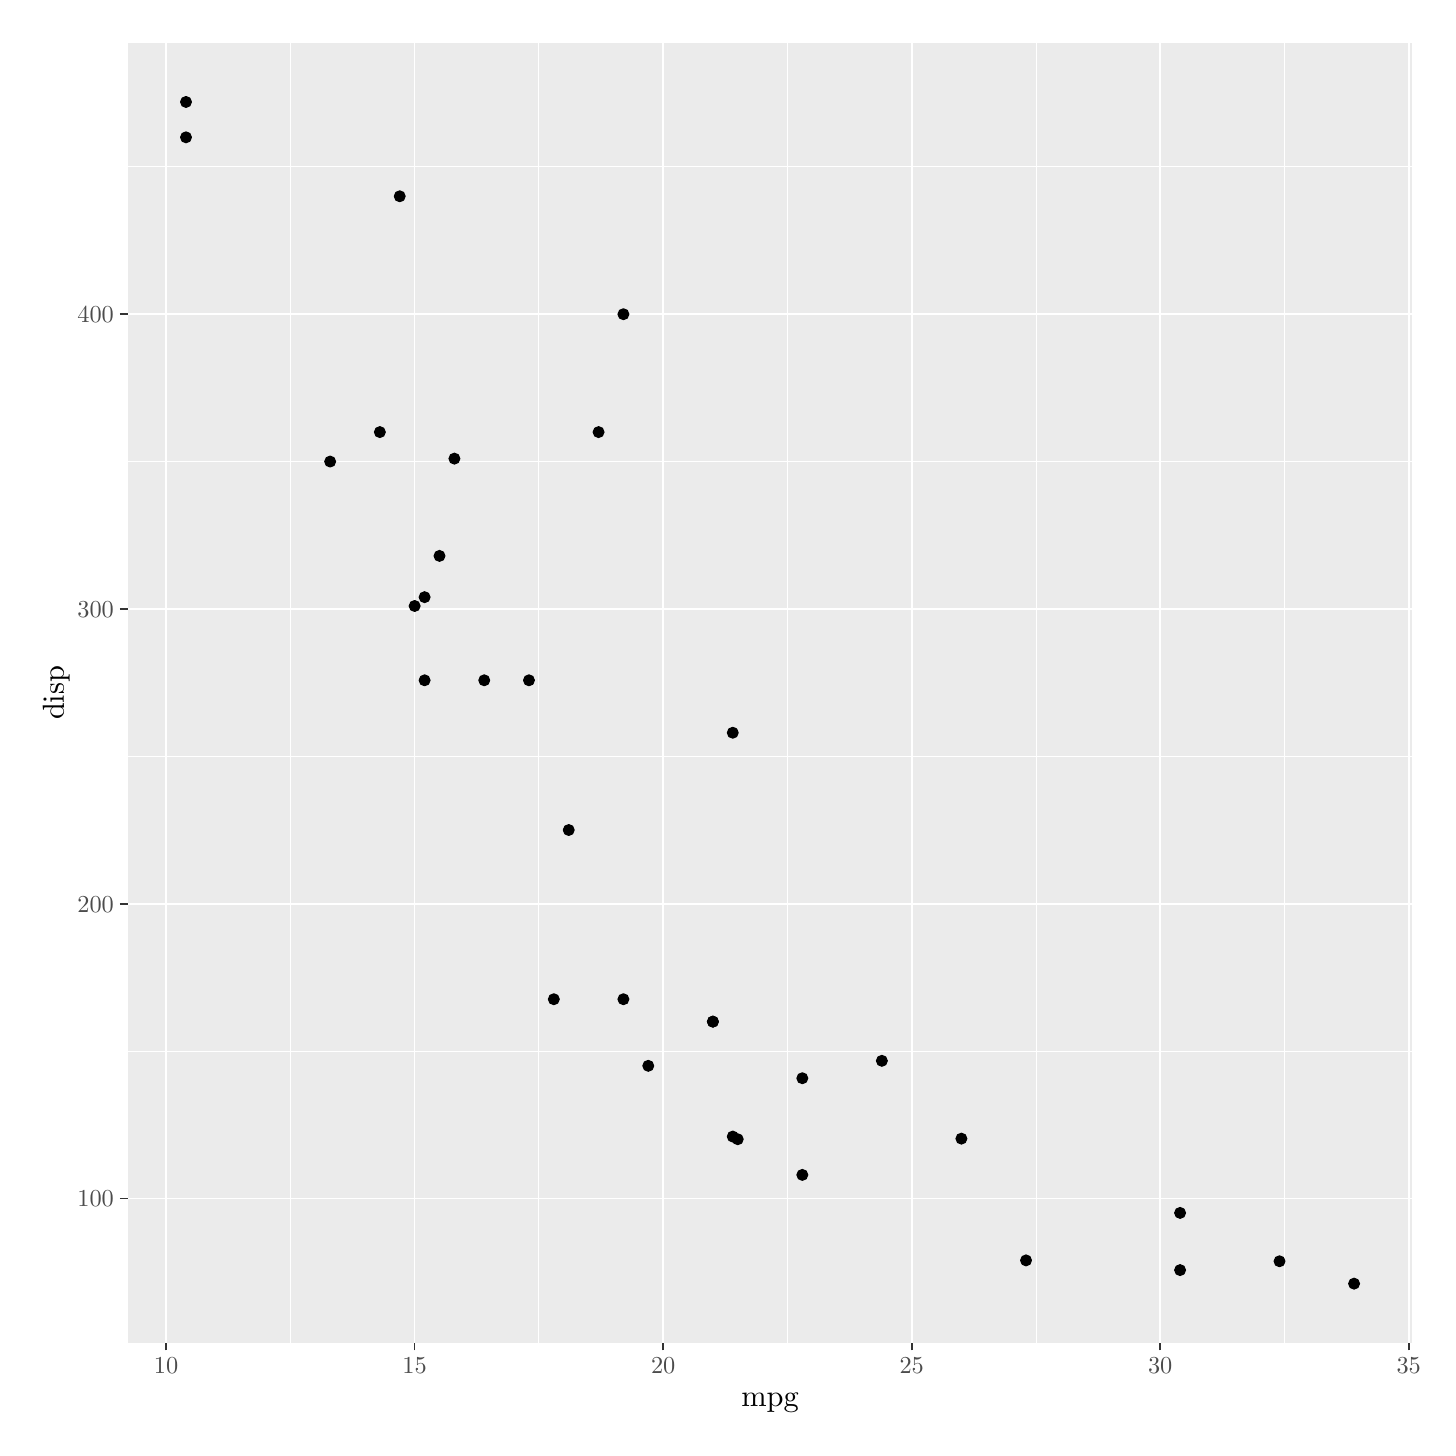
\begin{tikzpicture}[x=1pt,y=1pt]
\definecolor{fillColor}{RGB}{255,255,255}
\path[use as bounding box,fill=fillColor,fill opacity=0.00] (0,0) rectangle (505.89,505.89);
\begin{scope}
\path[clip] (  0.00,  0.00) rectangle (505.89,505.89);
\definecolor{drawColor}{RGB}{255,255,255}
\definecolor{fillColor}{RGB}{255,255,255}

\path[draw=drawColor,line width= 0.6pt,line join=round,line cap=round,fill=fillColor] (  0.00,  0.00) rectangle (505.89,505.89);
\end{scope}
\begin{scope}
\path[clip] ( 36.11, 30.69) rectangle (500.39,500.39);
\definecolor{fillColor}{gray}{0.92}

\path[fill=fillColor] ( 36.11, 30.69) rectangle (500.39,500.39);
\definecolor{drawColor}{RGB}{255,255,255}

\path[draw=drawColor,line width= 0.3pt,line join=round] ( 36.11,136.07) --
    (500.39,136.07);

\path[draw=drawColor,line width= 0.3pt,line join=round] ( 36.11,242.58) --
    (500.39,242.58);

\path[draw=drawColor,line width= 0.3pt,line join=round] ( 36.11,349.10) --
    (500.39,349.10);

\path[draw=drawColor,line width= 0.3pt,line join=round] ( 36.11,455.61) --
    (500.39,455.61);

\path[draw=drawColor,line width= 0.3pt,line join=round] ( 94.93, 30.69) --
    ( 94.93,500.39);

\path[draw=drawColor,line width= 0.3pt,line join=round] (184.73, 30.69) --
    (184.73,500.39);

\path[draw=drawColor,line width= 0.3pt,line join=round] (274.54, 30.69) --
    (274.54,500.39);

\path[draw=drawColor,line width= 0.3pt,line join=round] (364.34, 30.69) --
    (364.34,500.39);

\path[draw=drawColor,line width= 0.3pt,line join=round] (454.14, 30.69) --
    (454.14,500.39);

\path[draw=drawColor,line width= 0.6pt,line join=round] ( 36.11, 82.82) --
    (500.39, 82.82);

\path[draw=drawColor,line width= 0.6pt,line join=round] ( 36.11,189.33) --
    (500.39,189.33);

\path[draw=drawColor,line width= 0.6pt,line join=round] ( 36.11,295.84) --
    (500.39,295.84);

\path[draw=drawColor,line width= 0.6pt,line join=round] ( 36.11,402.35) --
    (500.39,402.35);

\path[draw=drawColor,line width= 0.6pt,line join=round] ( 50.03, 30.69) --
    ( 50.03,500.39);

\path[draw=drawColor,line width= 0.6pt,line join=round] (139.83, 30.69) --
    (139.83,500.39);

\path[draw=drawColor,line width= 0.6pt,line join=round] (229.64, 30.69) --
    (229.64,500.39);

\path[draw=drawColor,line width= 0.6pt,line join=round] (319.44, 30.69) --
    (319.44,500.39);

\path[draw=drawColor,line width= 0.6pt,line join=round] (409.24, 30.69) --
    (409.24,500.39);

\path[draw=drawColor,line width= 0.6pt,line join=round] (499.04, 30.69) --
    (499.04,500.39);
\definecolor{drawColor}{RGB}{0,0,0}
\definecolor{fillColor}{RGB}{0,0,0}

\path[draw=drawColor,line width= 0.4pt,line join=round,line cap=round,fill=fillColor] (247.60,146.72) circle (  1.96);

\path[draw=drawColor,line width= 0.4pt,line join=round,line cap=round,fill=fillColor] (247.60,146.72) circle (  1.96);

\path[draw=drawColor,line width= 0.4pt,line join=round,line cap=round,fill=fillColor] (279.92, 91.34) circle (  1.96);

\path[draw=drawColor,line width= 0.4pt,line join=round,line cap=round,fill=fillColor] (254.78,251.11) circle (  1.96);

\path[draw=drawColor,line width= 0.4pt,line join=round,line cap=round,fill=fillColor] (206.29,359.75) circle (  1.96);

\path[draw=drawColor,line width= 0.4pt,line join=round,line cap=round,fill=fillColor] (195.51,215.96) circle (  1.96);

\path[draw=drawColor,line width= 0.4pt,line join=round,line cap=round,fill=fillColor] (127.26,359.75) circle (  1.96);

\path[draw=drawColor,line width= 0.4pt,line join=round,line cap=round,fill=fillColor] (308.66,132.56) circle (  1.96);

\path[draw=drawColor,line width= 0.4pt,line join=round,line cap=round,fill=fillColor] (279.92,126.27) circle (  1.96);

\path[draw=drawColor,line width= 0.4pt,line join=round,line cap=round,fill=fillColor] (215.27,154.82) circle (  1.96);

\path[draw=drawColor,line width= 0.4pt,line join=round,line cap=round,fill=fillColor] (190.12,154.82) circle (  1.96);

\path[draw=drawColor,line width= 0.4pt,line join=round,line cap=round,fill=fillColor] (164.98,270.06) circle (  1.96);

\path[draw=drawColor,line width= 0.4pt,line join=round,line cap=round,fill=fillColor] (181.14,270.06) circle (  1.96);

\path[draw=drawColor,line width= 0.4pt,line join=round,line cap=round,fill=fillColor] (143.43,270.06) circle (  1.96);

\path[draw=drawColor,line width= 0.4pt,line join=round,line cap=round,fill=fillColor] ( 57.21,479.04) circle (  1.96);

\path[draw=drawColor,line width= 0.4pt,line join=round,line cap=round,fill=fillColor] ( 57.21,466.26) circle (  1.96);

\path[draw=drawColor,line width= 0.4pt,line join=round,line cap=round,fill=fillColor] (134.44,444.96) circle (  1.96);

\path[draw=drawColor,line width= 0.4pt,line join=round,line cap=round,fill=fillColor] (452.35, 60.13) circle (  1.96);

\path[draw=drawColor,line width= 0.4pt,line join=round,line cap=round,fill=fillColor] (416.42, 56.94) circle (  1.96);

\path[draw=drawColor,line width= 0.4pt,line join=round,line cap=round,fill=fillColor] (479.29, 52.04) circle (  1.96);

\path[draw=drawColor,line width= 0.4pt,line join=round,line cap=round,fill=fillColor] (256.58,104.23) circle (  1.96);

\path[draw=drawColor,line width= 0.4pt,line join=round,line cap=round,fill=fillColor] (148.81,315.01) circle (  1.96);

\path[draw=drawColor,line width= 0.4pt,line join=round,line cap=round,fill=fillColor] (143.43,300.10) circle (  1.96);

\path[draw=drawColor,line width= 0.4pt,line join=round,line cap=round,fill=fillColor] (109.30,349.10) circle (  1.96);

\path[draw=drawColor,line width= 0.4pt,line join=round,line cap=round,fill=fillColor] (215.27,402.35) circle (  1.96);

\path[draw=drawColor,line width= 0.4pt,line join=round,line cap=round,fill=fillColor] (360.75, 60.45) circle (  1.96);

\path[draw=drawColor,line width= 0.4pt,line join=round,line cap=round,fill=fillColor] (337.40,104.44) circle (  1.96);

\path[draw=drawColor,line width= 0.4pt,line join=round,line cap=round,fill=fillColor] (416.42, 77.60) circle (  1.96);

\path[draw=drawColor,line width= 0.4pt,line join=round,line cap=round,fill=fillColor] (154.20,350.16) circle (  1.96);

\path[draw=drawColor,line width= 0.4pt,line join=round,line cap=round,fill=fillColor] (224.25,130.75) circle (  1.96);

\path[draw=drawColor,line width= 0.4pt,line join=round,line cap=round,fill=fillColor] (139.83,296.91) circle (  1.96);

\path[draw=drawColor,line width= 0.4pt,line join=round,line cap=round,fill=fillColor] (254.78,105.19) circle (  1.96);
\end{scope}
\begin{scope}
\path[clip] (  0.00,  0.00) rectangle (505.89,505.89);
\definecolor{drawColor}{gray}{0.30}

\node[text=drawColor,anchor=base east,inner sep=0pt, outer sep=0pt, scale=  0.88] at ( 31.16, 79.79) {100};

\node[text=drawColor,anchor=base east,inner sep=0pt, outer sep=0pt, scale=  0.88] at ( 31.16,186.30) {200};

\node[text=drawColor,anchor=base east,inner sep=0pt, outer sep=0pt, scale=  0.88] at ( 31.16,292.81) {300};

\node[text=drawColor,anchor=base east,inner sep=0pt, outer sep=0pt, scale=  0.88] at ( 31.16,399.32) {400};
\end{scope}
\begin{scope}
\path[clip] (  0.00,  0.00) rectangle (505.89,505.89);
\definecolor{drawColor}{gray}{0.20}

\path[draw=drawColor,line width= 0.6pt,line join=round] ( 33.36, 82.82) --
    ( 36.11, 82.82);

\path[draw=drawColor,line width= 0.6pt,line join=round] ( 33.36,189.33) --
    ( 36.11,189.33);

\path[draw=drawColor,line width= 0.6pt,line join=round] ( 33.36,295.84) --
    ( 36.11,295.84);

\path[draw=drawColor,line width= 0.6pt,line join=round] ( 33.36,402.35) --
    ( 36.11,402.35);
\end{scope}
\begin{scope}
\path[clip] (  0.00,  0.00) rectangle (505.89,505.89);
\definecolor{drawColor}{gray}{0.20}

\path[draw=drawColor,line width= 0.6pt,line join=round] ( 50.03, 27.94) --
    ( 50.03, 30.69);

\path[draw=drawColor,line width= 0.6pt,line join=round] (139.83, 27.94) --
    (139.83, 30.69);

\path[draw=drawColor,line width= 0.6pt,line join=round] (229.64, 27.94) --
    (229.64, 30.69);

\path[draw=drawColor,line width= 0.6pt,line join=round] (319.44, 27.94) --
    (319.44, 30.69);

\path[draw=drawColor,line width= 0.6pt,line join=round] (409.24, 27.94) --
    (409.24, 30.69);

\path[draw=drawColor,line width= 0.6pt,line join=round] (499.04, 27.94) --
    (499.04, 30.69);
\end{scope}
\begin{scope}
\path[clip] (  0.00,  0.00) rectangle (505.89,505.89);
\definecolor{drawColor}{gray}{0.30}

\node[text=drawColor,anchor=base,inner sep=0pt, outer sep=0pt, scale=  0.88] at ( 50.03, 19.68) {10};

\node[text=drawColor,anchor=base,inner sep=0pt, outer sep=0pt, scale=  0.88] at (139.83, 19.68) {15};

\node[text=drawColor,anchor=base,inner sep=0pt, outer sep=0pt, scale=  0.88] at (229.64, 19.68) {20};

\node[text=drawColor,anchor=base,inner sep=0pt, outer sep=0pt, scale=  0.88] at (319.44, 19.68) {25};

\node[text=drawColor,anchor=base,inner sep=0pt, outer sep=0pt, scale=  0.88] at (409.24, 19.68) {30};

\node[text=drawColor,anchor=base,inner sep=0pt, outer sep=0pt, scale=  0.88] at (499.04, 19.68) {35};
\end{scope}
\begin{scope}
\path[clip] (  0.00,  0.00) rectangle (505.89,505.89);
\definecolor{drawColor}{RGB}{0,0,0}

\node[text=drawColor,anchor=base,inner sep=0pt, outer sep=0pt, scale=  1.10] at (268.25,  7.64) {mpg};
\end{scope}
\begin{scope}
\path[clip] (  0.00,  0.00) rectangle (505.89,505.89);
\definecolor{drawColor}{RGB}{0,0,0}

\node[text=drawColor,rotate= 90.00,anchor=base,inner sep=0pt, outer sep=0pt, scale=  1.10] at ( 13.08,265.54) {disp};
\end{scope}
\end{tikzpicture}
